\documentclass[lualatex, aspectratio=169]{beamer}

\usetheme{Data61}

\title{Aboleth}
\subtitle{Bayesian Neural Networks and More}
\author{Dan Steinberg}
\date{April 11, 2018}
\institute{Inference Systems Engineering}

\usepackage{fontspec}
\usepackage{color}
\usepackage{minted}  % needs pygments package
\usemintedstyle{friendly}
\usepackage{unicode-math}
\usefonttheme{serif}

\defaultfontfeatures{Ligatures=TeX}
\setmainfont{Open Sans}
\setsansfont{Open Sans}
% \setmonofont{Inconsolata}
\setmonofont{Ubuntu Mono}
% \setmathfont{DejaVu Math Tex Gyre}
% \setmathfont{XITS Math}

% Math
\renewcommand{\v}[1]{\mathbf{#1}}
\renewcommand{\d}{\,\mathrm{d}}
\newcommand{\T}{^\top}
\newcommand{\vp}[1]{\mathbf{#1}^{\prime}}
\newcommand{\h}[1]{\hat{#1}}
\newcommand{\cov}[2]{\mathrm{Cov}(#1,#2)}
\newcommand{\hil}{\mathscr{H}}
\newcommand{\reals}{\mathbb{R}}
\newcommand{\complexs}{\mathbb{C}}
\newcommand{\dprod}[2]{{\langle #1, #2 \rangle}}
\newcommand{\expec}[1]{\mathbb{E}\!\left[{#1}\right]}
\newcommand{\argmin}{\operatornamewithlimits{argmin}}
\newcommand{\pd}[2]{\frac{\partial#1}{\partial#2}}
\newcommand{\norm}[1]{\|#1\|}
\newcommand{\query}[1]{{#1}^{*}}


% Text
\newcommand{\imp}[1]{\textcolor{Data61 green}{\textbf{#1}}}

%%%%%%%%%%%%%%%%%%%%%%%
% global renew commands
%%%%%%%%%%%%%%%%%%%%%%%
\makeatletter
\def\gnewcommand{\g@star@or@long\new@command}
\def\grenewcommand{\g@star@or@long\renew@command}
\def\g@star@or@long#1{% 
  \@ifstar{\let\l@ngrel@x\global#1}{\def\l@ngrel@x{\long\global}#1}}
\makeatother
%%%%%%%%%%%%%%%%%%%%%%%%%%%
% end global renew commands
%%%%%%%%%%%%%%%%%%%%%%%%%%%

\let\oldint\int
\grenewcommand\int{\oldint\!}
\grenewcommand{\epsilon}{\varepsilon}

\let\oldemptyset\emptyset
\let\emptyset\varnothing

\newtheorem{prp}{Proposition}[section]
\newtheorem{thm}{Theorem}[section]

\theoremstyle{definition}
\newtheorem{dfn}{Definition}[section]

\newcommand{\sidenote}[1]{
  \marginline{{\fontsize{8}{8}\selectfont
    \begin{spacing}{1}
#1
    \end{spacing} }}
}



\begin{document}

\maketitle

\begin{frame}{Outline}
  \begin{enumerate}
    \item Background: Supervised learning to Bayesian neural networks
    \item Aboleth:
    \begin{itemize}
      \item{Why another NN framework?}
      \item{How its interface compares to other frameworks}
      \item{Some of the internals}
      \item{Examples}
    \end{itemize}
  \end{enumerate}
\end{frame}


\section{Supervised Learning \\ to Bayesian NNs}


\begin{frame}{Supervised learning}
  \begin{itemize}
    \item <1-> $\v{x}$ is a vector of covariates or features, $y$ a target 
    \item <2-> There exists an unknown function, $f$, that maps the covariates to the targets with some error,
      \begin{align*}
        y = f(\v{x}) + \epsilon
      \end{align*}
    \item <3> E.g. Houses have attributes, $\v{x}$, and market forces, $f$, control prices, $y$. 
    \item <4-> \emph{Supervised ML}: learn an approximation of this function, $h$, using examples,
      \begin{align*}
        y_i \approx h(\v{x}_i) \quad \text{for all} \quad \{(y_1, \v{x}_1), (y_2, \v{x}_2), \ldots,
          (y_N, \v{x}_N) \}
      \end{align*}
    \item <5> E.g. Historical house sales data.
  \end{itemize}
\end{frame}


\begin{frame}{Supervised learning}
  \begin{itemize}
    \item Usually we choose a class of $h$ with parameters, $\theta$,
    \item learning is \imp{optimisation} of these parameters.
  \end{itemize}
  % \begin{align*}
  %   \hat{\theta} = \argmin_\theta \frac{1}{N} \sum^N_{i=1} \mathcal{L}\!\left(y_i, h(\v{x}_i, \theta)\right),
  % \end{align*}
  % where $\mathcal{L}$ is a \imp{loss} or \imp{error} function.

  % \pause
  
  % \hspace{1cm}
  \begin{columns}
    \column{0.51\pagewidth}
    For example, find the $\theta$ that minimises the sum of squared errors
    \begin{align*}
      \hat\theta = \argmin_{\theta} \frac{1}{N} \sum^N_{i=1} (y_i - h(\v{x}_i, \theta))^2
    \end{align*}
    \column{0.3\pagewidth}
    \begin{figure}
      \includegraphics[width=0.3\pagewidth]{assets/gd.png}
    \end{figure}
  \end{columns}

\end{frame}


\begin{frame}{Prediction}
  Once we have learned $h$, we want to use it to \imp{predict} $\query{y}$ for \imp{new}, \imp{unseen} instances of $\query{\v{x}}$,
  \begin{align*}
    \expec{\query{y}} = h(\query{\v{x}}, \hat{\theta}).
  \end{align*}
\end{frame}


\begin{frame}{Regression example}

  \begin{description}
    \item[True function] $f(x) = \sin(x)$
    \item[Observations] $y_i = f(x_i) + \epsilon_i, \quad \epsilon_i \sim \mathcal{N}(0, 0.1)$
  \end{description}

  \begin{figure}
    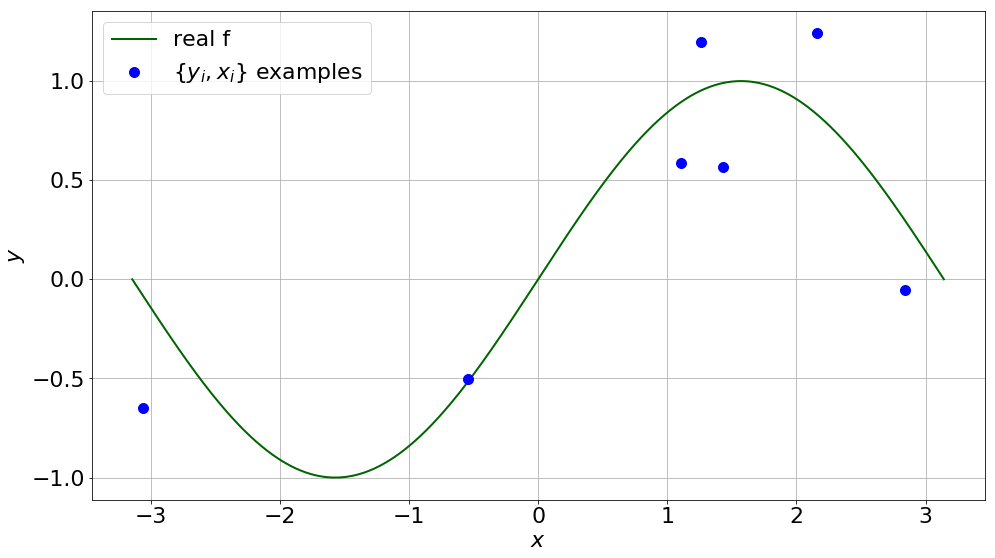
\includegraphics[width=0.6\pagewidth]{assets/regress.png}
  \end{figure}

\end{frame}


% \begin{frame}{Fit a line}

%   \begin{description}
%     \item[Model] $h(x) = w_0 + w_1 x$
%     \item[Objective] $\argmin_{\v{w}} \frac{1}{N} \sum^N_{i=1} \|y_i - h(x_i)\|^2_2$ 
%   \end{description}

%   \begin{figure}
%     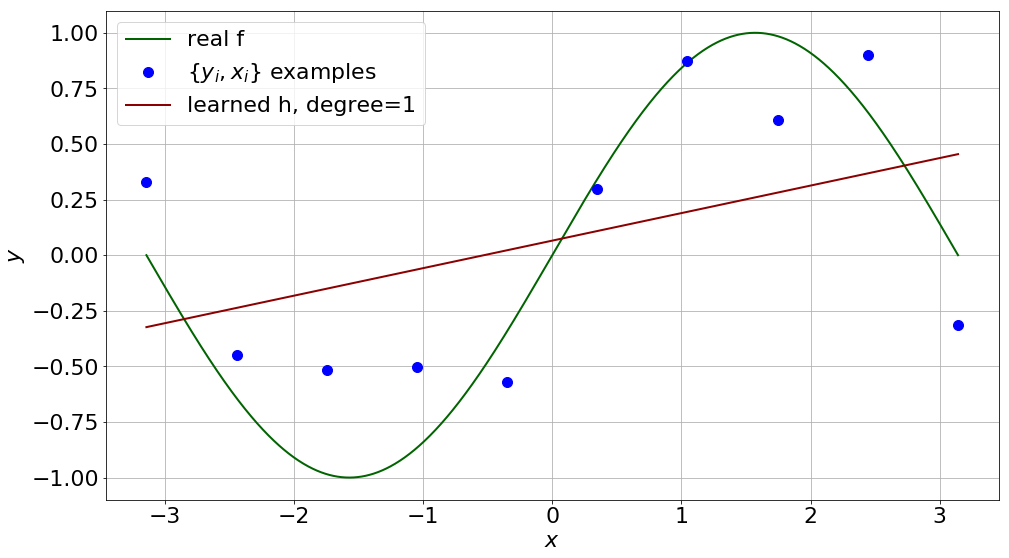
\includegraphics[width=0.5\pagewidth]{assets/poly1.png}
%   \end{figure}

%   Under-fitting --- bad generalisation/interpolation.

% \end{frame}


\begin{frame}{Fit a degree-3 polynomial}

  \begin{description}
    \item[Model] $h(x, \v{w}) = w_0 + w_1 x + w_2 x^2 + w_3 x^3$
    \item[Objective] $\argmin_{\v{w}} \frac{1}{N} \sum^N_{i=1} (y_i - h(x_i, \v{w}) )^2$ 
  \end{description}

  \begin{figure}
    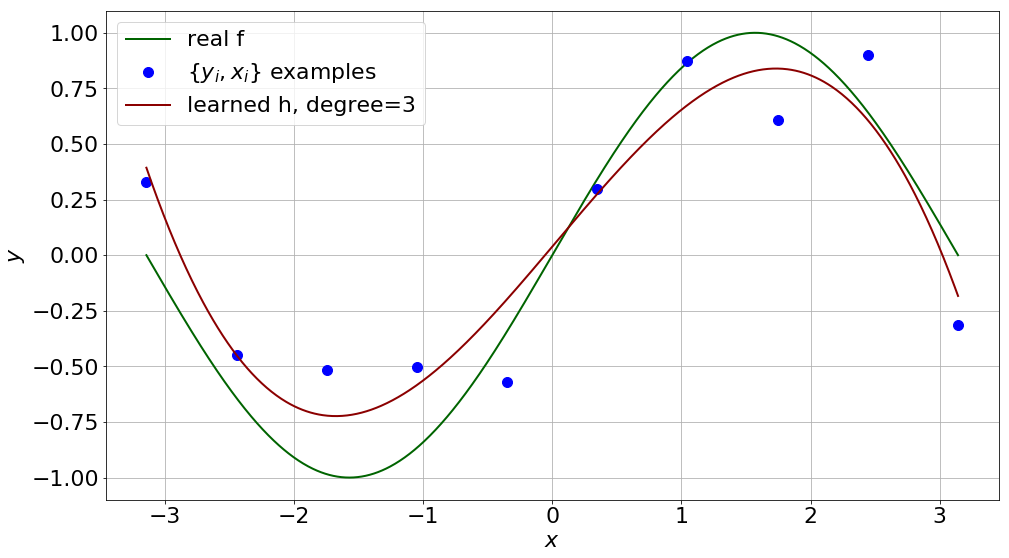
\includegraphics[width=0.6\pagewidth]{assets/poly3.png}
  \end{figure}

\end{frame}


\begin{frame}{Linear Models}

  So we saw a polynomial is one class of model, e.g.:
  \begin{align*}
    h(x, \v{w}) &= w_0 + w_1 x + w_2 x^2 + w_3 x^3 \\
                &= \begin{bmatrix} w_0 & w_1 & w_2 & w_3 \end{bmatrix}
                   \begin{bmatrix} 1 \\ x \\ x^2 \\ x^3 \end{bmatrix} \\
                   &= \v{w}\T \text{Poly}_3(x)
  \end{align*}
  This is part of a general class of models we call \imp{linear} models,
  \begin{align*}
    h(\v{x}, \v{w}) &= \v{w}\T \phi(\v{x})
  \end{align*}
  where $\phi$ is some function.

\end{frame}


\begin{frame}{Neural Nets}
  
  Neural nets generalise this class of linear models with \imp{non-linearities} ($\sigma$) and \imp{function composition}:
  \begin{itemize}
    \item 0 hidden layers: $\NN{0}{\v{x}} = \sigma_0( \v{W}_0\v{x} )$
    \item 1 hidden layer: $\NN{1}{\v{x}} = \sigma_1(\v{W}_1 \sigma_0( \v{W}_0 \v{x} ))$
    \item L hidden layers: $\NN{L}{\v{x}} = \sigma_L(\v{W}_L \sigma_{L-1}(\v{W}_{L-1} \ldots \sigma( \v{W}_0 \v{x} )))$
  \end{itemize}

  \begin{figure}
    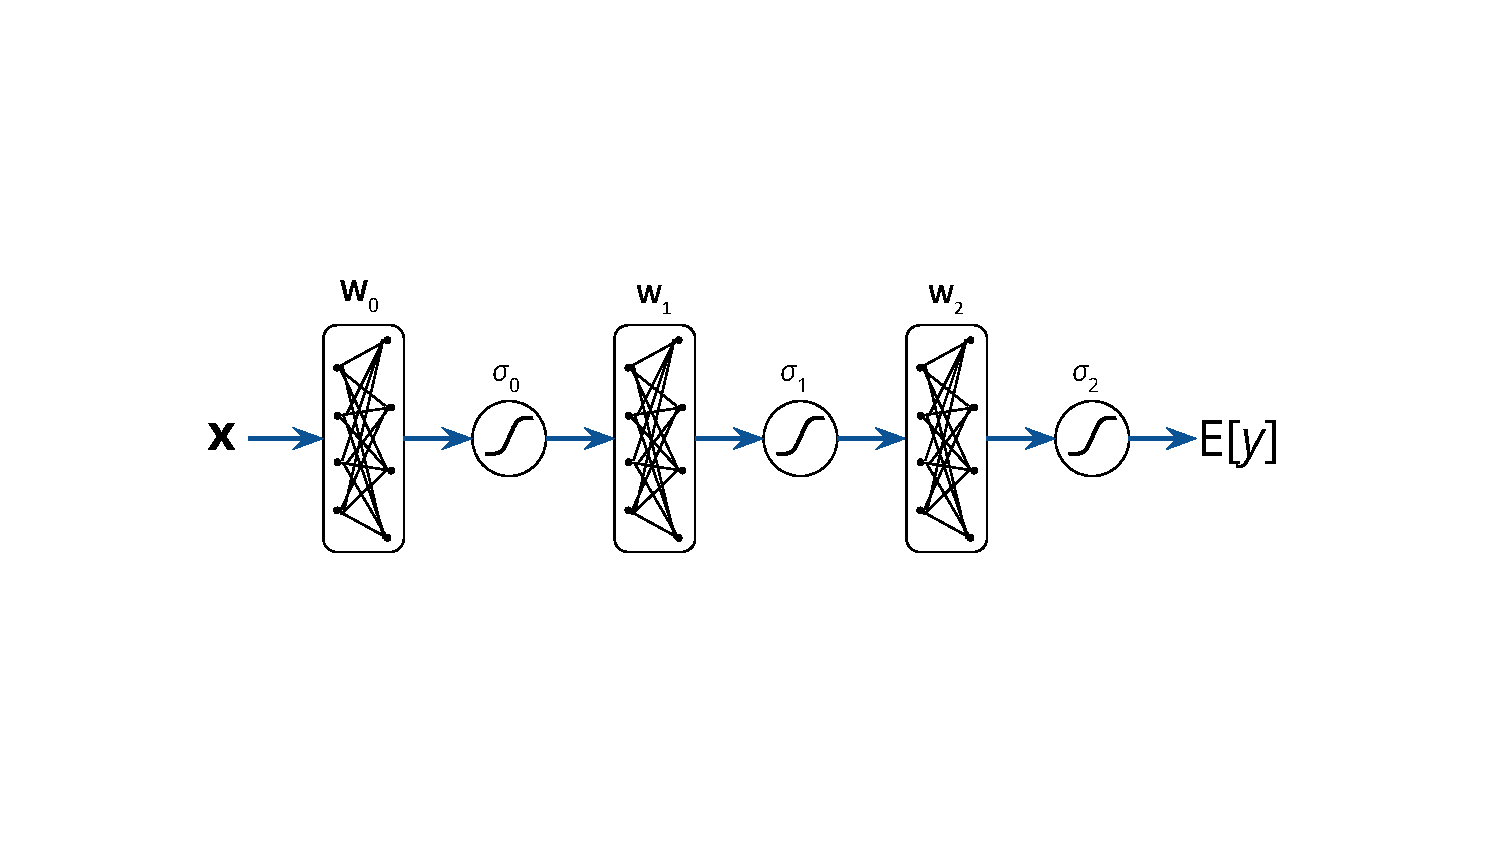
\includegraphics[page=1, trim={3cm 4.5cm 3.5cm 4.5cm}, clip, width=0.5\pagewidth]{assets/pictures.pdf}
  \end{figure}
  
\end{frame}


\begin{frame}{Why this representation?}

  Neural nets can represent any function! But \ldots
  \begin{itemize}
    \item The more complex the function, the `wider' the layers have to be (for a given depth).
    \item Or we can use (exponentially) `narrower' and \imp{deeper} nets!
  \end{itemize}

  Nice demo: \href{https://playground.tensorflow.org}{TensorFlow Playground}
  \begin{figure}
    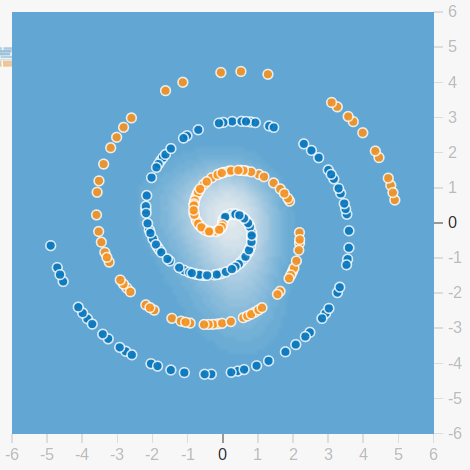
\includegraphics[width=0.2\pagewidth]{assets/swirl.png}
  \end{figure}


\end{frame}


\begin{frame}{TensorFlow Playground --- Spiral}

  \begin{figure}
    \centering
    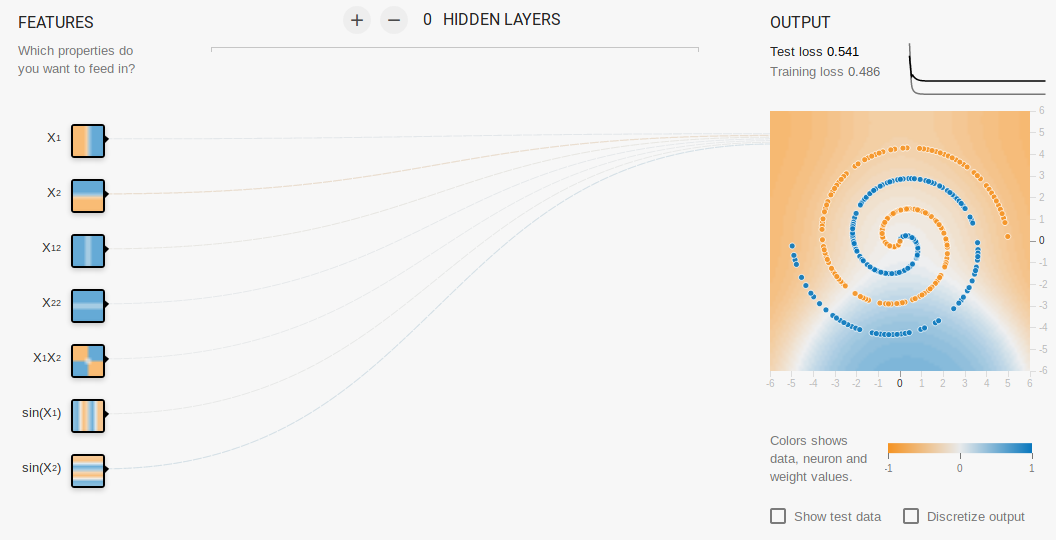
\includegraphics[height=0.75\pageheight]{assets/0-hidden.png}
  \end{figure}

\end{frame}


\begin{frame}{TensorFlow Playground --- Spiral}

  \begin{figure}
    \centering
    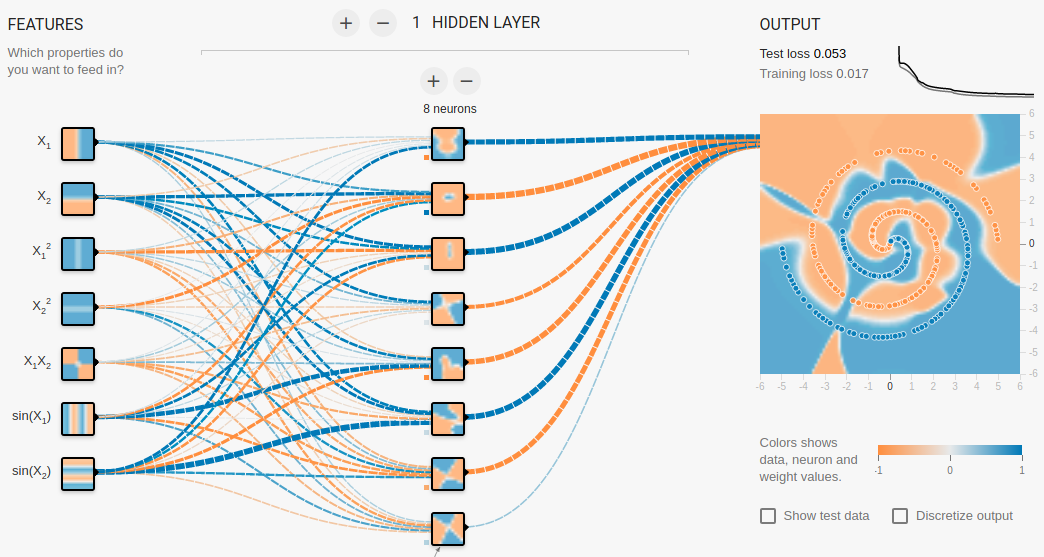
\includegraphics[height=0.75\pageheight]{assets/1-hidden.png}
  \end{figure}

\end{frame}


\begin{frame}{TensorFlow Playground --- Spiral}

  \begin{figure}
    \centering
    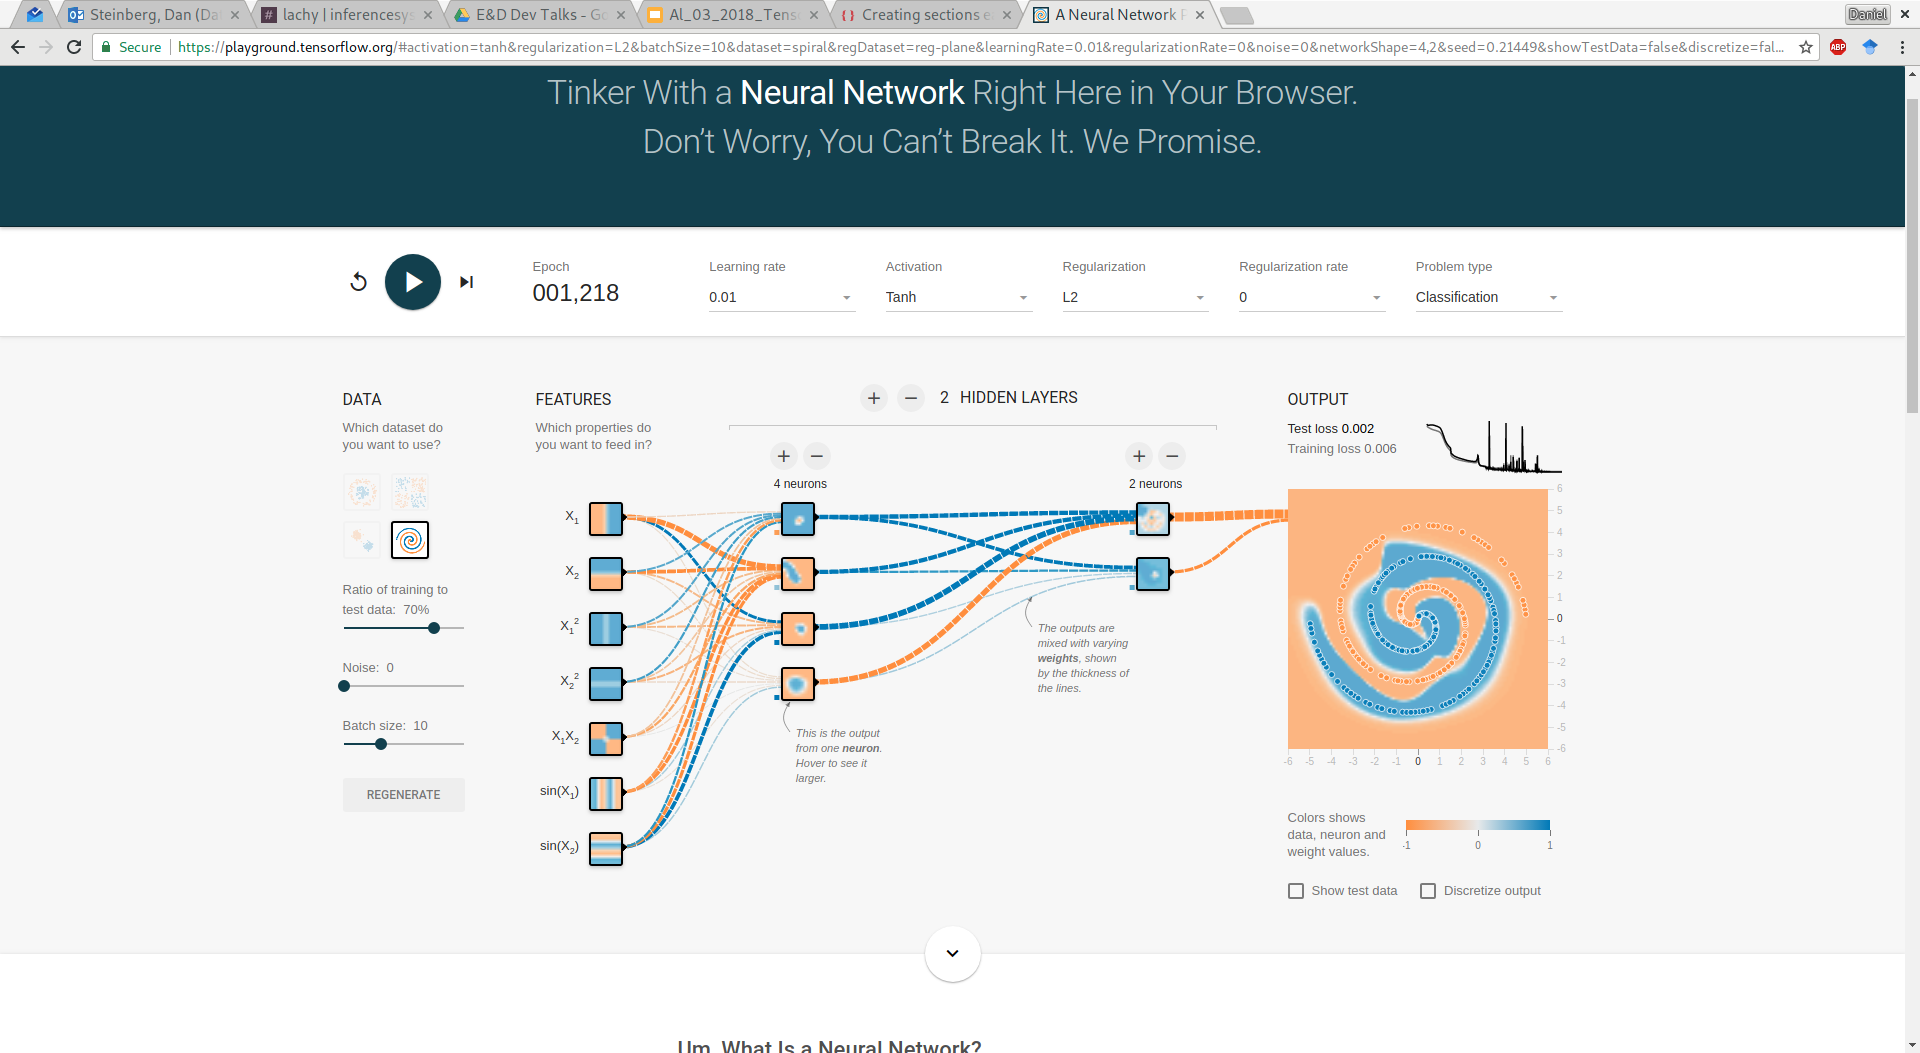
\includegraphics[height=0.75\pageheight]{assets/2-hidden.png}
  \end{figure}

\end{frame}


\begin{frame}{TensorFlow Playground --- Spiral}

  \begin{figure}
    \centering
    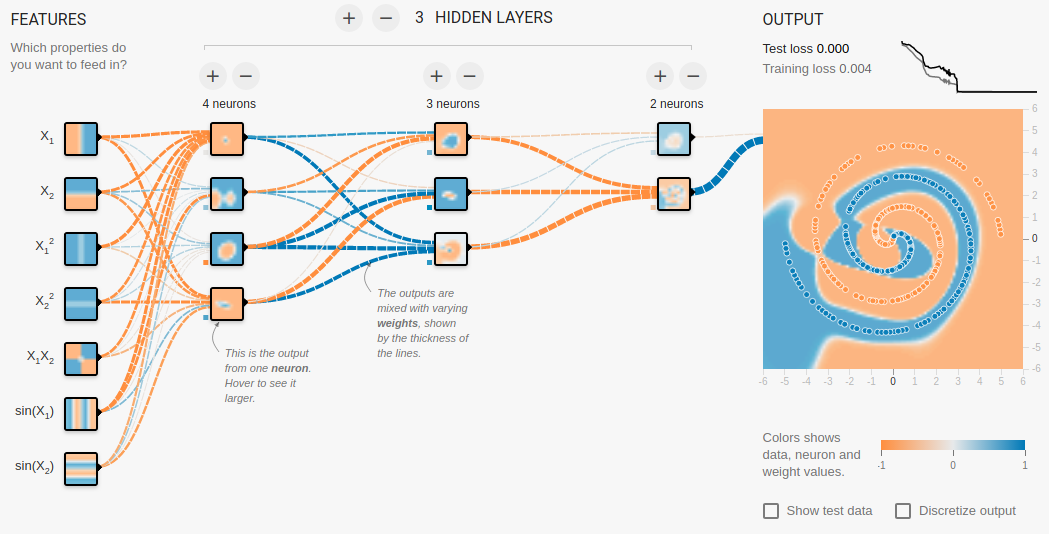
\includegraphics[height=0.75\pageheight]{assets/3-hidden.png}
  \end{figure}

\end{frame}


\begin{frame}{Neural Nets and Abstraction}

  \begin{figure}
    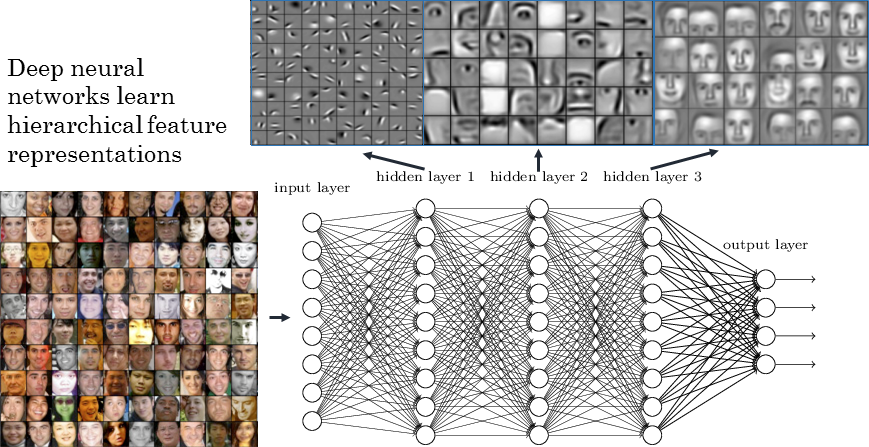
\includegraphics[width=0.7\pagewidth]{assets/abstraction.png}
    \caption{https://www.rsipvision.com/exploring-deep-learning/}
  \end{figure}

\end{frame}

% \begin{frame}{Fit a Degree-9 Polynomial}

%   \begin{description}
%     \item[Model] $h(x) = w_0 + w_1 x + \ldots + w_9 x^9$
%     \item[Objective] $\argmin_{\v{w}} \frac{1}{N} \sum^N_{i=1} \|y_i - h(x_i)\|^2_2$ 
%   \end{description}

%   \begin{figure}
%     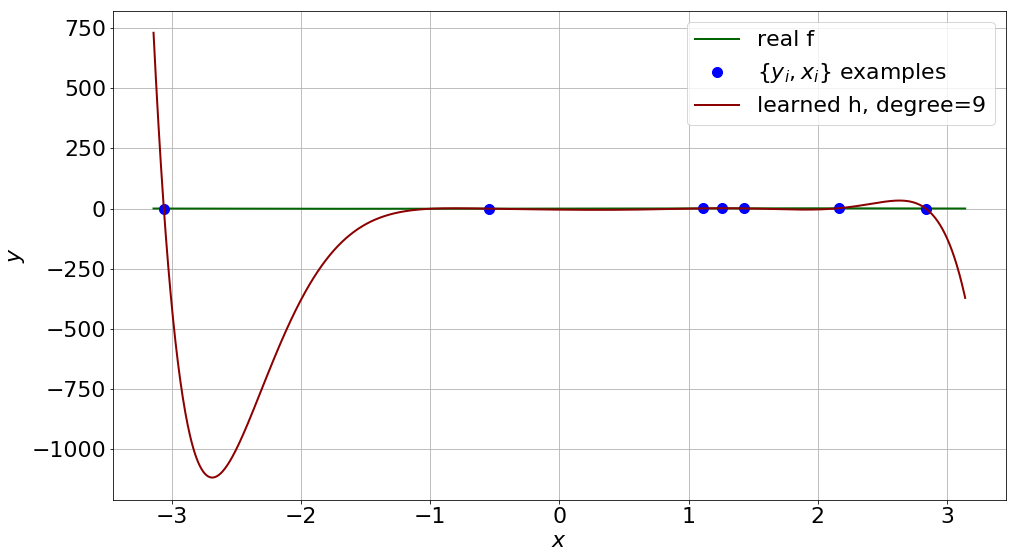
\includegraphics[width=0.5\pagewidth]{assets/poly9.png}
%   \end{figure}

%   Over fitting --- fits points exactly, but bad for interpolation.
% \end{frame}


% \begin{frame}{Regularisation}
%   TODO: why regularisation is important

%   TODO: what the learning objective looks like with regularisation
% \end{frame}


\begin{frame}{Probabilistic Prediction}

  So far we've just looked at predictors that give us $\expec{\query{y} | h(\query{\v{x}}, \hat\theta)}$ --- don't explicitly model uncertainty.

  \begin{description}[\leftmargin=0cm]
    \item[Maximum Likelihood] methods:
      \begin{align*}
        p(\query{y} | h(\query{\v{x}}, \hat\theta))
      \end{align*}
      model the uncertainty in the \imp{targets} (point estimate parameters).
    \item[Bayesian] methods:
      \begin{align*}
        \frac{1}{S} \sum_s p(\query{y} | h(\query{\v{x}}, \theta_s)),
          \qquad \theta_s \sim p(\theta | \{(y_1, \v{x}_1), (y_2, \v{x}_2), \ldots \})
      \end{align*}
      also model the uncertainty in the \imp{model parameters}.
  \end{description}
\end{frame}


\begin{frame}{Probabilistic Prediction}

  Here is the same $\sin$ function fit using a Bayesian predictor (GP):
  \begin{figure}
    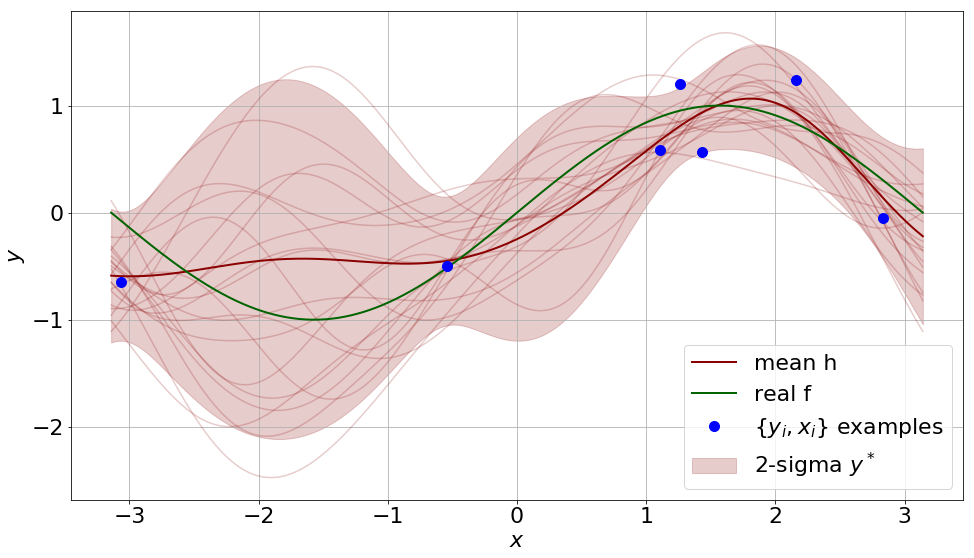
\includegraphics[width=0.6\pagewidth]{assets/probabilistic.png}
  \end{figure}
  \imp{Note}: where there isn't much data, uncertainty grows \ldots

\end{frame}


\begin{frame}{Why Probabilistic Prediction?}

  \begin{columns}
    \column{0.5\pagewidth}
    Great for decision making, e.g.
    \begin{itemize}
      \item \emph{Don't use this prediction because the model is uncertain} --- good when predicting something about people.
      \item \emph{Getting more data} --- where should I sample next to make the model more confident?
    \end{itemize}
    \column{0.4\pagewidth}
    \begin{figure}
      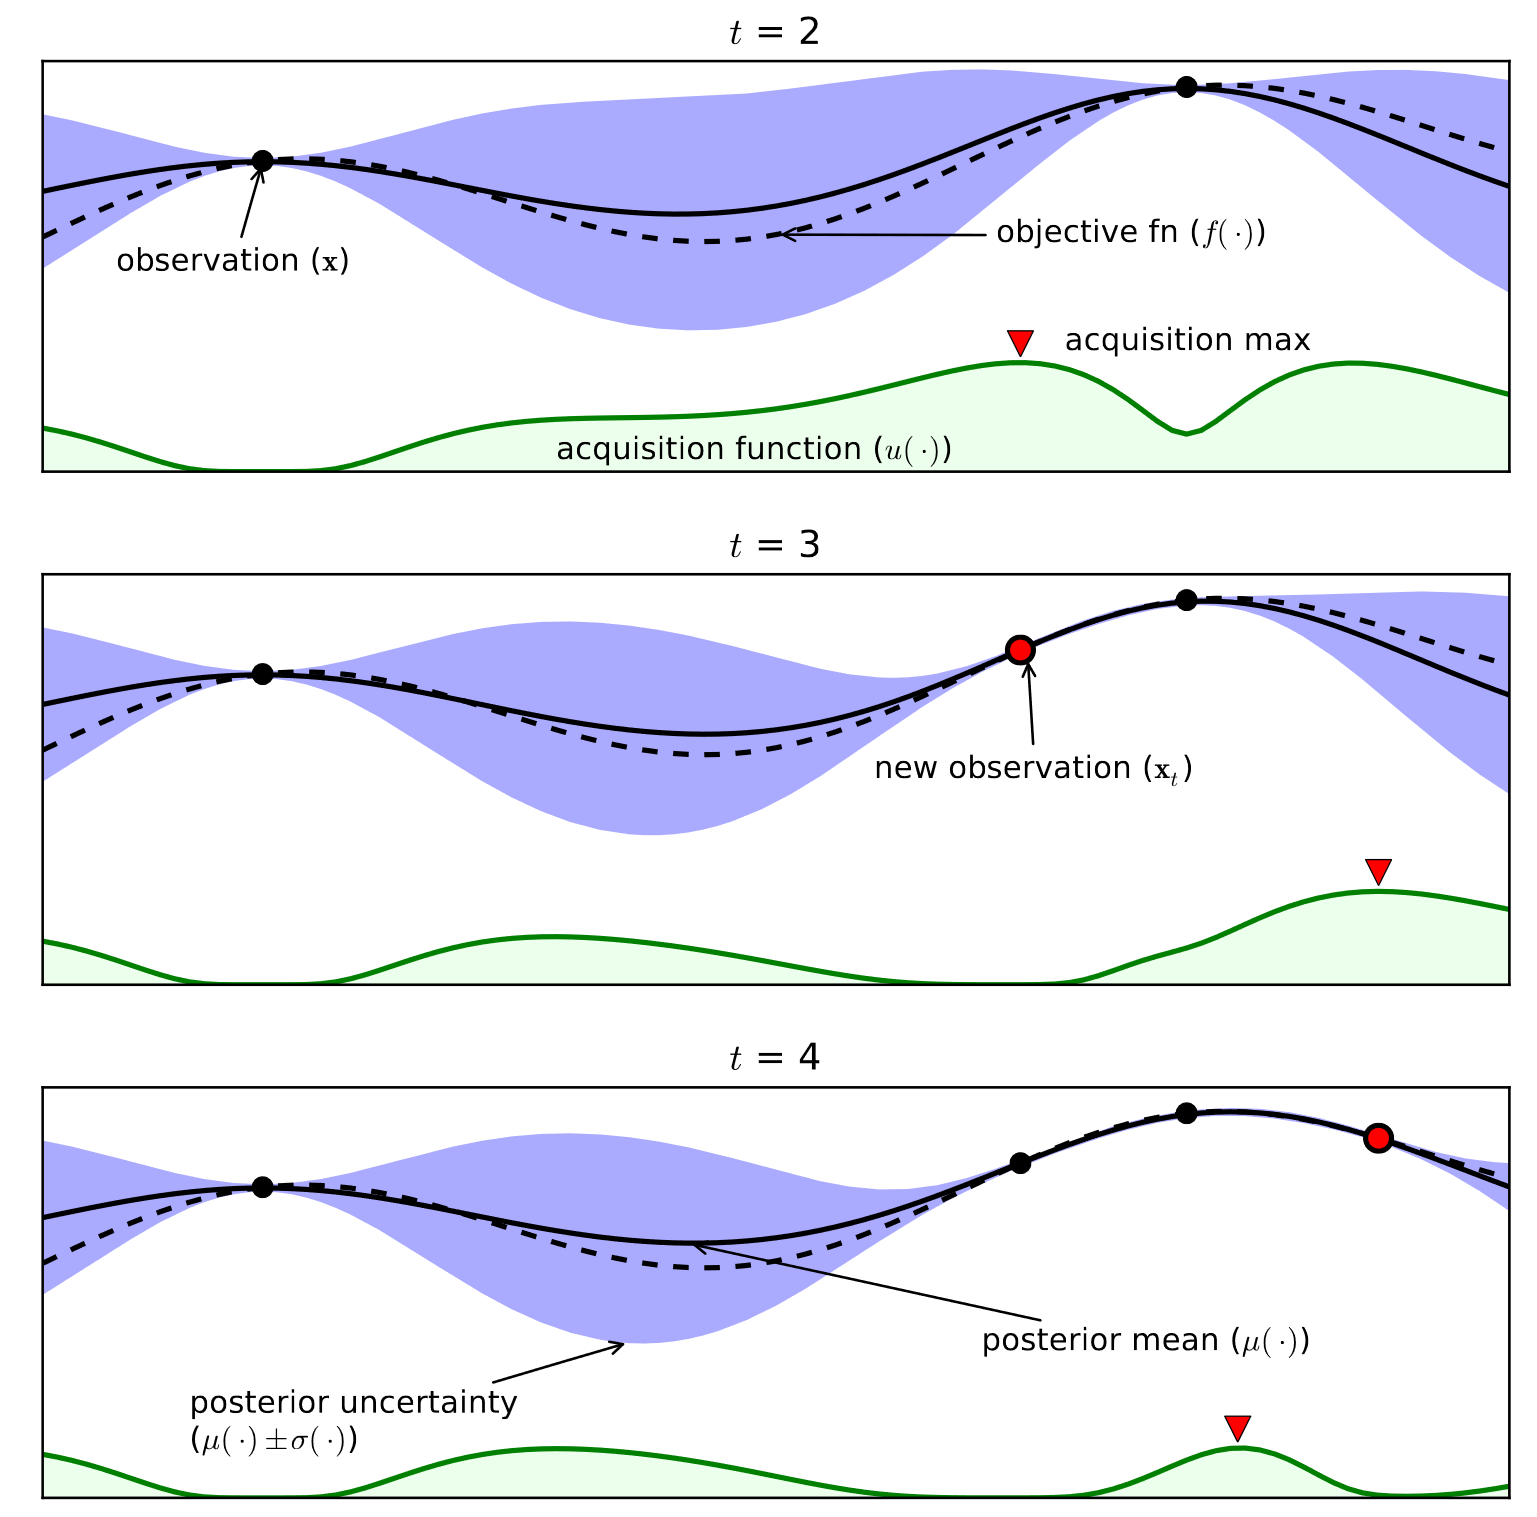
\includegraphics[width=0.36\pagewidth]{assets/bayesopt.png}
      \caption{\href{https://towardsdatascience.com/shallow-understanding-on-bayesian-optimization-324b6c1f7083}{Bayesian optimisation}}.
    \end{figure}
  \end{columns}

\end{frame}


\begin{frame}{Bayesian Neural Nets}

  \begin{figure}
    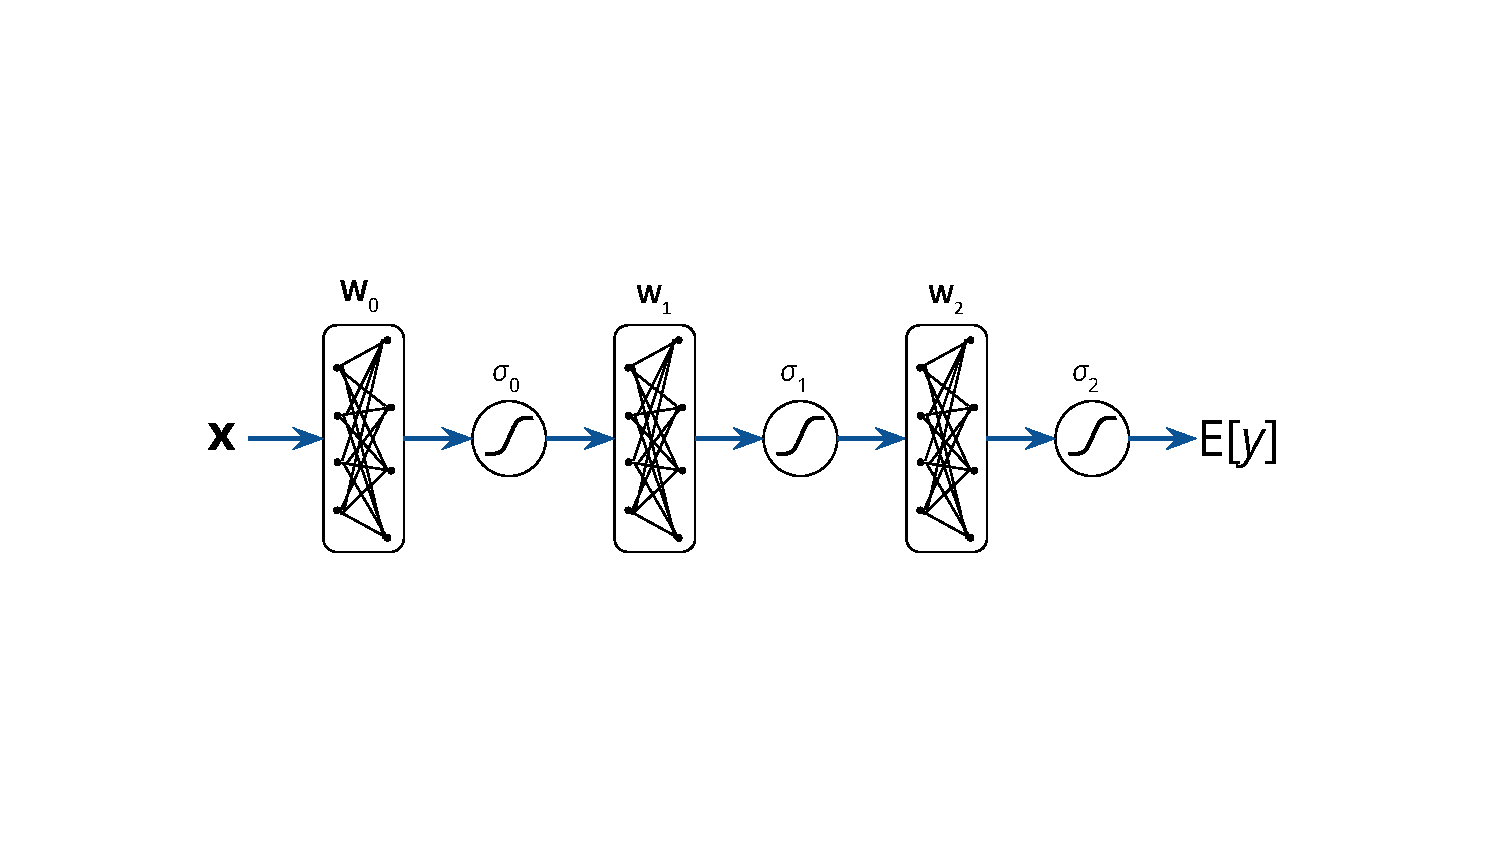
\includegraphics[page=1, trim={3cm 4.5cm 3cm 4.5cm}, clip, width=0.6\pagewidth]{assets/pictures.pdf}
    \includegraphics[page=3, trim={3cm 4.5cm 3cm 4.5cm}, clip, width=0.6\pagewidth]{assets/pictures.pdf}
  \end{figure}

  Bayesian NNs propagate \imp{random samples of their weights} through the network, making a stochastic neural network. 
  % This has to be \imp{built into the computational graph}.

\end{frame}


\begin{frame}{Bayesian Neural Nets}

  \begin{columns}
    \column{0.35\pagewidth}
    Learning involves \imp{function composition} (evaluating the NN), and \imp{accumulation} (weight regularisation). 

    \hspace{1cm}

    For a BNN, its samples have to be \imp{built into the computational graph} since they are part of the \imp{learning objective}.

    \hspace{1cm}

    This motivates the need for a specialised framework for BNNs.

    \column{0.6\pagewidth}
    \begin{figure}
      \includegraphics[page=2, trim={3cm 2.5cm 0cm 4.5cm}, clip, width=0.6\pagewidth]{assets/pictures.pdf}
      \includegraphics[page=4, trim={3cm 2.5cm 0cm 4.5cm}, clip, width=0.6\pagewidth]{assets/pictures.pdf}
    \end{figure}
  \end{columns}

\end{frame}


\section{Aboleth}

\begin{frame}{Why do we need another NN framework?}

  \begin{itemize}
    \item \imp{TensorFlow, PyTorch, MXNet, \ldots} --- too low level (a lot of boiler-plate)
    \item \imp{Keras} --- not inherently Bayesian
    \item \imp{Edward, PyMC3} --- probabilistic programming, a bit too general
    \item \imp{ZhuSuan} --- Like Edward, but with less functionality and worse design
  \end{itemize}

  \hspace{1cm}

  So, there isn't really a \emph{simple to use and extendable} library specifically for Bayesian NNs (\ldots in python 3)

\end{frame}


\begin{frame}{Aboleth Features}
  \begin{columns}
    \column{0.7\pagewidth}
    \begin{itemize}
      \item Built on TensorFlow (great for deployments, monitoring etc)
      \item Bayesian layers (Dense, convolutional, embedding)
      \item Simple interface, simple to extend/interoperate with underlying TensorFlow
      \item Large scale Gaussian process approximation
      \item Multiple inputs: imputing layers, embedding layers etc
      \item Compatible with Keras
      \item \imp{Stochastic variational Bayes}$^1$ inference (and SGD)
    \end{itemize}
    \column{0.25\pagewidth}
    \begin{figure}
      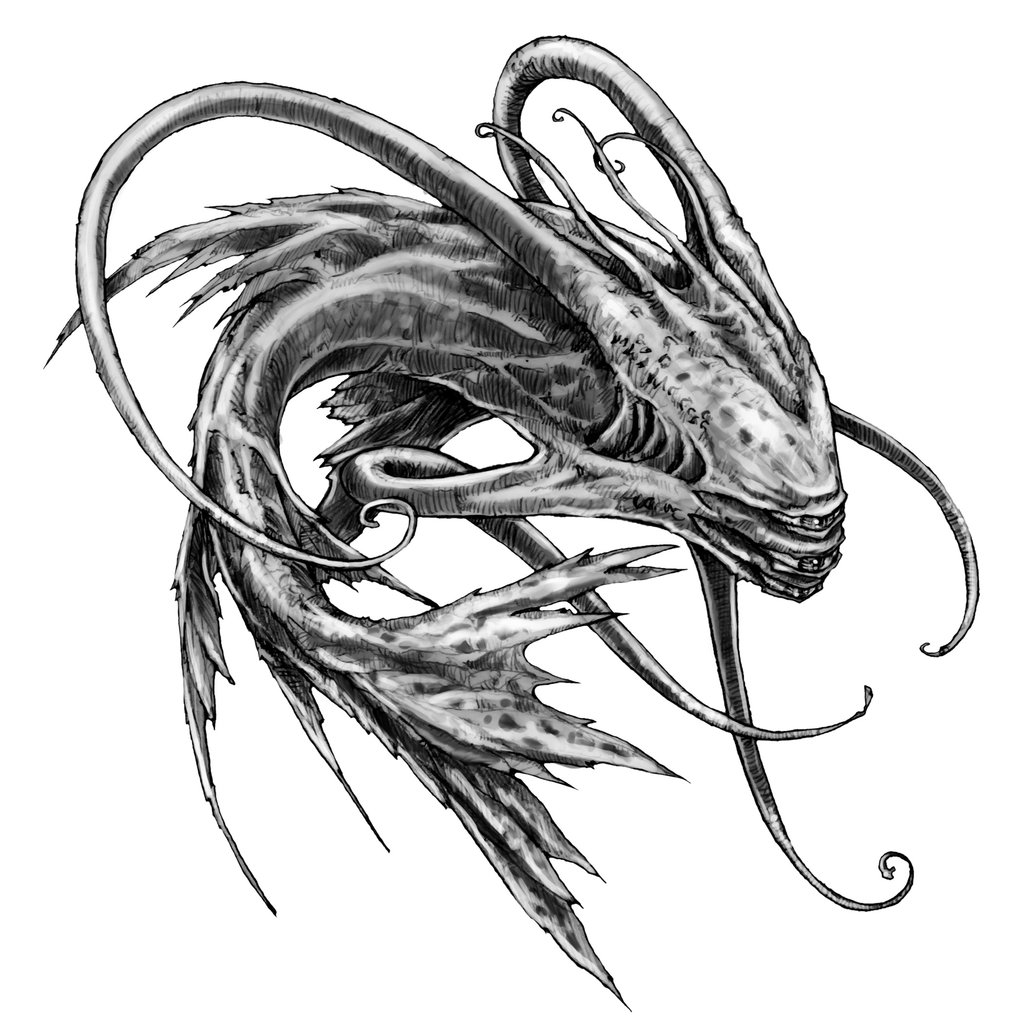
\includegraphics[width=0.25\pagewidth]{assets/aboleth.jpg}
    \end{figure}
  \end{columns}
  \tiny{$^1$Kingma, D. P. and Welling, M. Auto-encoding variational Bayes. In ICLR, 2014}
\end{frame}


\begin{frame}{Interface comparison}
  Let's implement a one hidden layer Bayesian NN:
  \begin{itemize}
    \item $\v{x}$ and $y$ are one dimensional
    \item $\v{W}_0 \in \reals^{1 \times 20}$
    \item $\v{W}_1 \in \reals^{20 \times 1}$
  \end{itemize}
    \begin{figure}
      \includegraphics[page=5, trim={3cm 4.5cm 10cm 4.5cm}, clip, width=0.6\pagewidth]{assets/pictures.pdf}
    \end{figure}
\end{frame}


\begin{frame}[fragile]{Interface comparison --- Edward}
  Let's implement a one hidden layer Bayesian NN in Edward (\url{http://edwardlib.org/}):
  
  \begin{minted}[linenos, mathescape]{python}

    from edward.models import Normal

    W_0 = Normal(loc=tf.zeros([1, 20]), scale=tf.ones([1, 20]))
    W_1 = Normal(loc=tf.zeros([20, 1]), scale=tf.ones([20, 1]))

    def neural_network(x):
        h = tf.tanh(tf.matmul(x, W_0))
        h = tf.matmul(h, W_1)
        return tf.reshape(h, [-1])

    y = Normal(loc=neural_network(x_train), scale=0.1)

  \end{minted}
\end{frame}


\begin{frame}[fragile]{Interface comparison --- Edward}
  Continuing \ldots
  
  \begin{minted}[linenos, mathescape]{python}

    import edward as ed

    qW_0 = Normal(loc=tf.get_variable("qW_0/loc", [1, 20]),
              scale=tf.nn.softplus(tf.get_variable("qW_0/scale", [1, 20])))
    qW_1 = Normal(loc=tf.get_variable("qW_1/loc", [20, 1]),
              scale=tf.nn.softplus(tf.get_variable("qW_1/scale", [20, 1])))

    inference = ed.KLqp({W_0: qW_0, W_1: qW_1}, data={y: y_train})
    inference.run(n_iter=1000)
  \end{minted}
\end{frame}


\begin{frame}{Interface comparison --- Edward}

  Some remarks:
  \begin{itemize}
    \item Quite a general probabilistic framework (great for prototyping Bayesian models)
    \item As a result, probably requires a bit too much boilerplate for BNNs
    \item Make sure you get the dimensions of your layers right!
    \item PyMC3 is quite similar
  \end{itemize}

\end{frame}


\begin{frame}{Interface comparison --- ZhuSuan}
  Let's implement a one hidden layer Bayesian NN in ZhuSuan (\url{https://github.com/thu-ml/zhusuan})

  \hspace{1cm}

  Too long --- click \href{http://zhusuan.readthedocs.io/en/latest/tutorials/bayesian_nn.html}{here}\ldots  

  \hspace{1cm}

  Some remarks:
  \begin{itemize}
    \item What is the probability of getting this right the first time?
    \item Why wouldn't I use Edward or PyMC3?
  \end{itemize}

\end{frame}


\begin{frame}[fragile]{Interface comparison --- Aboleth}

  \begin{minted}[linenos, mathescape, fontsize=\scriptsize]{python}
  import tensorflow as tf
  import aboleth as ab

  # Construct the network, no data needed
  net = (
    ab.InputLayer(name="X", n_samples=5) >>   # how we assign data, and # samples 
    ab.DenseVariational(output_dim=20) >>
    ab.Activation(tf.tanh) >>
    ab.DenseVariational(output_dim=1)
    )

  # Build the computational graph for the net, attach data x_train
  nn, reg = net(X=x_train)

  # Now make the training objective, attach targets
  likelihood = tf.distributions.Normal(loc=nn, scale=0.1).log_prob(y_train)
  loss = ab.elbo(likelihood, reg, N_training)

  # Standard TensorFlow training code here

  \end{minted}

\end{frame}


\begin{frame}{Interface comparison --- Aboleth}
  
  \begin{itemize}
    \item \texttt{>>} implements the NN \imp{function composition}, and \imp{regularisation accumulation}
    \begin{itemize}
      \item Tony has told us this is an instance of a \imp{writer monad}
      \item Each layer composes itself with previous layers, and accumulates its complexity penalty
    \end{itemize}
    \item We don't need to know the shape of the input (unlike Keras), or the inputs to any layers, only the output shapes!
    \begin{itemize}
      \item the input shapes are lazily evaluated when data/placeholders are input
    \end{itemize}
  \end{itemize}

\end{frame}


\begin{frame}[fragile]{Layers in Aboleth}

  \begin{minted}[linenos, mathescape, fontsize=\scriptsize]{python}
  class Layer:
      """Layer base class."""

      def __call__(self, X):
          """Construct the subgraph for this layer."""
          Net, KL = self._build(X)
          return Net, KL

      def _build(self, X):
          """Implement graph construction. Should be over-ridden."""
          return X, 0.0

      def __rshift__(self, other):
          """Implement layer composition, other(self(x))."""
          return LayerComposite(self, other)

  \end{minted}

  \begin{itemize}
    \item Usually you just need to subclass \texttt{Layer}, and implement \texttt{\_build, \_\_init\_\_}.
    \item We also have \texttt{MultiLayers}, which take in key-word argument pairs
  \end{itemize}
\end{frame}


\begin{frame}{Aboleth Examples}
  Lets look at how we can use Aboleth for regression, we have some docs here:
  \url{http://aboleth.readthedocs.io/en/stable/tutorials/some_regressors.html}

  \begin{figure}
    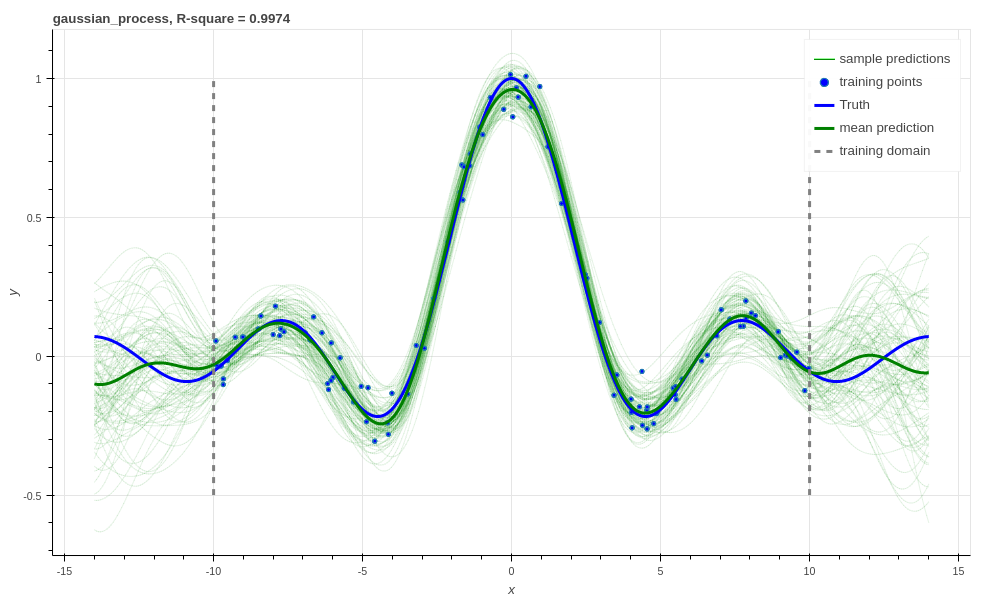
\includegraphics[width=0.6\pagewidth]{assets/gpr.png}
  \end{figure}

\end{frame}


\begin{frame}[fragile]{Use Aboleth for your \emph{whole} pipeline}

  Learn values to impute missing data as part of the network
  \begin{columns}
    \column{0.6\pagewidth}
    \begin{minted}[mathescape, fontsize=\scriptsize]{python}
        # Construct the network, no data needed
        data_input = ab.InputLayer(name="X", n_samples=5)
        mask_input = ab.MaskInputLayer(name="M")

        net = (
            ab.LearnedScalarImpute(data_input, mask_input) >>
            ab.DenseVariational(output_dim=1, full=True)
        )

        # Build the computational graph for the net, attach data X, M
        nn, reg = net(X=x_data, M=x_missing_mask)
        # ...
    \end{minted}
    \column{0.35\pagewidth}
    \begin{itemize}
      \item We now have two input layers, one for data, and one for a missingness mask
      \item We then attach the data and mask
    \end{itemize}
  \end{columns}

\end{frame}


\begin{frame}[fragile]{Combine Networks}
  
  \begin{columns}
    \column{0.55\pagewidth}
    \begin{minted}[mathescape, fontsize=\scriptsize]{python}
    # Ordinal data
    ord_net = (
        ab.InputLayer(name="Xord", n_samples=5) >>
        ab.DenseVariational(output_dim=10)
    )

    # Categorical data
    cat_net = (
        ab.InputLayer(name="Xcat", n_samples=5) >>
        ab.EmbedVariational(output_dim=10, n_categories=100)
    )

    # Join them
    net = (
        ab.Concat(cat_net, ord_net) >>
        ab.Activation(tf.nn.relu)  >>
        ab.DenseVariational(output_dim=1)
    )

    nn, reg = net(Xcat=x_categorical, Xord=x_ordinal)
    \end{minted}
    \column{0.4\pagewidth}
    \begin{itemize}
      \item We can create separate embedding pipelines then join (concatenate) them
      \item We can add imputing to this
      \item We also have tools to replicate the categorical embedding for more categorical features
    \end{itemize}
  \end{columns}
\end{frame}


\begin{frame}{Please dive in!}

  \begin{itemize}
    \item Repo: \url{https://github.com/data61/aboleth}
    \item Docs: \url{http://aboleth.readthedocs.io/en/stable/?badge=stable}
    \item We've been using it for > 6 months on most projects
    \item Easy to deploy on Bracewell
    \item Lots of issues that we need help with!
  \end{itemize}

  \hspace{2cm}

  \imp{Thanks!}

  \hspace{2cm}

  \emph{Contributors}: Dan Steinberg, Lachlan McCalman, Louis Tiao, Simon O'Callaghan, Alistair Reid

  \{daniel.steinberg, lachlan.mccalman\}@data61.csiro.au

\end{frame}


\end{document}
